%!TEX root = ../report.tex

\newcommand\scalemath[2]{\scalebox{#1}{\mbox{\ensuremath{\displaystyle #2}}}}


\begin{document}
    \chapter{Evaluation and Experimental Result}
	\label{chap:evaluationandresult}
    Evaluation and experimental result chapter contains the metrics used to evaluate the conducted experiment and the discussion on the research questions. Results of research question is answered in the subsequent sections with listing of the result in a table. Three research questions answered in the section are the results of state of the art temporal fusion techniques, How are the results in comparison to each other and finally cross transfer the temporal fusion techniques from depth estimation to the semantic segmentation. The model is trained and evaluated on three datasets Scannet \cite{79_dai2017scannet}, Virtual kitti \cite{80_cabon2020vkitti2} and VIODE \cite{81_minodaRAL2021} datasets. 
    
    \section{Evaluation Metric}
    
    The proposed model needs to be validated to understand the impact of the newly trained model. To validate the model different evaluation metrics are proposed. The description of the proposed model is listed below.
    \subsection{Pixel Accuracy}
    
    Pixel accuracy is commonly defined as percent of pixels in a image correctly classified into a particular class. Accuracy is defined as below
    
    $
    {\bf Accuracy } = \scalemath{2}{\frac{TP+TN}{TP+TN+FP+FN}}
    $
    
    where
     
    $TP$ = True Positive 
    
    $TN$ = True Negative
    
    $FP$ = False Positive
    
    $FN$ = False Negative
    
    
    Per class mean pixel accuracy (mPA)
    
    Per class mean pixel accuracy is the average of pixel accuracies of all the classes.
    
    Pixel accuracy (PA) and Mean pixel accuracy (mPA) can also be defined as below \cite{84_ulku2022survey}
    
    $
    {\bf PA } = \scalemath{2}{\frac{\sum_{j=1}^{k} n_{jj}}{\sum_{j=1}^{k} t_j} }
    $
    
    $
    {\bf mPA } = \scalemath{2}{\frac{1}{k} \frac{\sum_{j=1}^{k} n_{jj}}{\sum_{j=1}^{k} t_j}}
    $
    
    where $n_{jj}$ is the total number of pixels both classified and labeled as class $j$. 
    
    \subsection{IoU}
    
    Intersection over Union (IoU) also known as the Jaccard index is a method to quantify the overlapping between the target mask and the predicted output. In other words, it is number of pixels common between the target and prediction masks by the total number of pixels exist between both the masks \cite{83_iou}. pictorial representation of the same is presented in Fig \ref{fig:IoU}
    
    \begin{figure}[h]
    	\centering
    	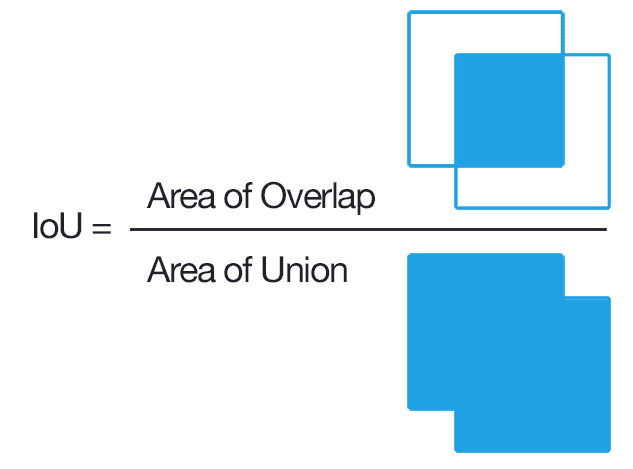
\includegraphics[width=12cm]{images/IoU.png}
    	\caption{IoU. Courtesy of \cite{82_iou}}
    	\label{fig:IoU}
    \end{figure}  
	
	IoU is calculated for each class separately and then averaged over all the classes to provide mean IoU.  
	
	$
	{\bf IoU} = \scalemath{2}{\frac{\sum_{j=1}^{k} n_{jj}}{\sum_{j=1}^{k} (n_{ij}+n_{ji}+n_{jj})}, i \neq j }
	$

	where $ n_{ij}$ is the pixels which are labeled as class i but classified as class j and $n_{ji}$ is the total number of pixels labeled as class j, but classified as class i. \cite{84_ulku2022survey}
	
	$
	{\bf mIoU} = \scalemath{2}{\frac{1}{k} \sum_{j=1}^k \frac{n_{ij}}{n_{ij}+n_{ji}+n_{jj}},  i \neq j }
	$
	
	Frequency weighted IoU (FwIoU). It is a metric derived from the mIoU which weighs each class importance depending on appearance frequency using $t_j$ \cite{84_ulku2022survey}
	
	$
	{\bf FwIoU} = \scalemath{2} {\frac{1}{\sum_{j=1}^k t_j} \sum_{j=1}^{k} t_j \frac{n_{jj}}{n_{ij}+n_{ji}+n_{jj}}, i \neq j }
	$
    
    
    \section{RQ1: What are the works on state-of-the-art temporal fusion?}
    \subsection{Experiment1.1: U-Net and W-Net model with single sequence data}
    \subsection{Experiment1.2: U-Net and W-Net model with two sequence data}
    \subsection{Experiment1.3: U-Net and W-Net model with three sequence data}
    \subsection{Experiment1.4: U-Net and W-Net model with four sequence data}
    \subsection{Experiment1.5: U-Net and W-Net model with all sequence data}
    \section{RQ2: How are the results from RQ1 compared with each other to perform temporal fusion?}
    \subsection{Experiment1.1: U-Net and W-Net model with single sequence data}
    \subsection{Experiment1.2: U-Net and W-Net model with two sequence data}
    \subsection{Experiment1.3: U-Net and W-Net model with three sequence data}
    \subsection{Experiment1.4: U-Net and W-Net model with four sequence data}
    \subsection{Experiment1.5: U-Net and W-Net model with all sequence data}
    \section{RQ3: How to cross-transfer the temporal fusion technique to semantic segmentation?}
    \subsection{Experiment1.1: U-Net vanilla model}
    
    U-net model is developed to categorize the biomedical images. Currently the model is used in the other application areas as well. The original network is mainly based on the data augmentation strategy. The network consist of a encoder and decoder along with the interconnection between different layers of encoder and decoder. The expanding path of the U-net model helps to capture the location of the objects in the image. The vanilla U-net model code is referenced from the Kaggle competition \cite{85_kag_challenge}. The result presented below is for vanilla U-net model trained on the scannet dataset \cite{79_dai2017scannet}. The model is trained for 300 epochs. The below figure \ref{fig:y_gt_vanilla} depicts the distribution of the pixel based on the classes. There are totally 41 classes [ \ref{table:Classes in scannet_1} , \ref{table:Classes in scannet_2} , \ref{table:Classes in scannet_3}] present in the entire Scannet datasets.        
    
    \newpage 
    
    \begin{center}
    	\begin{tabular}{ | l | p{12cm} |}
    		\hline
    		
    		\cellcolor{purple!30}Metric & \cellcolor{purple!30}Value \\ \hline
    		Pixel Accuracy & 0.5096 \\ \hline
    		Pixel Mean accuracy & 0.1907  \\ \hline
    		meanIOU & 0.1102 \\ \hline
    		IoU & [1.8345e-01, 5.6047e-01, 6.0881e-01, 1.6476e-01, 3.8241e-01, 1.1697e-01, 
    		2.3122e-02, 8.9410e-02, 2.5848e-01, 1.6661e-01, 2.0180e-03, 2.0504e-01, 
    		4.5985e-02,        nan, 4.2167e-02, 1.1143e-01, 2.3969e-01, 1.2545e-02, 
    		1.1324e-01, 2.7658e-03, 0.0000e+00, 7.0415e-02, 7.0606e-02, 0.0000e+00,  
    		0.0000e+00, 1.2208e-01, 1.4680e-02, 1.1862e-04, 2.2112e-04, 6.5610e-03, 
    		4.3742e-03,        nan, 7.6680e-02, 3.5784e-02, 1.1516e-01, 5.6912e-02, 
    		2.9310e-04, 3.7764e-02, 2.2634e-02, 1.1269e-01, 2.2094e-01] \\ \hline
    		FwIoU & 0.3531 \\ \hline
    		\hline
    	\end{tabular}
    \end{center}
	
	\begin{figure}
		\centering
		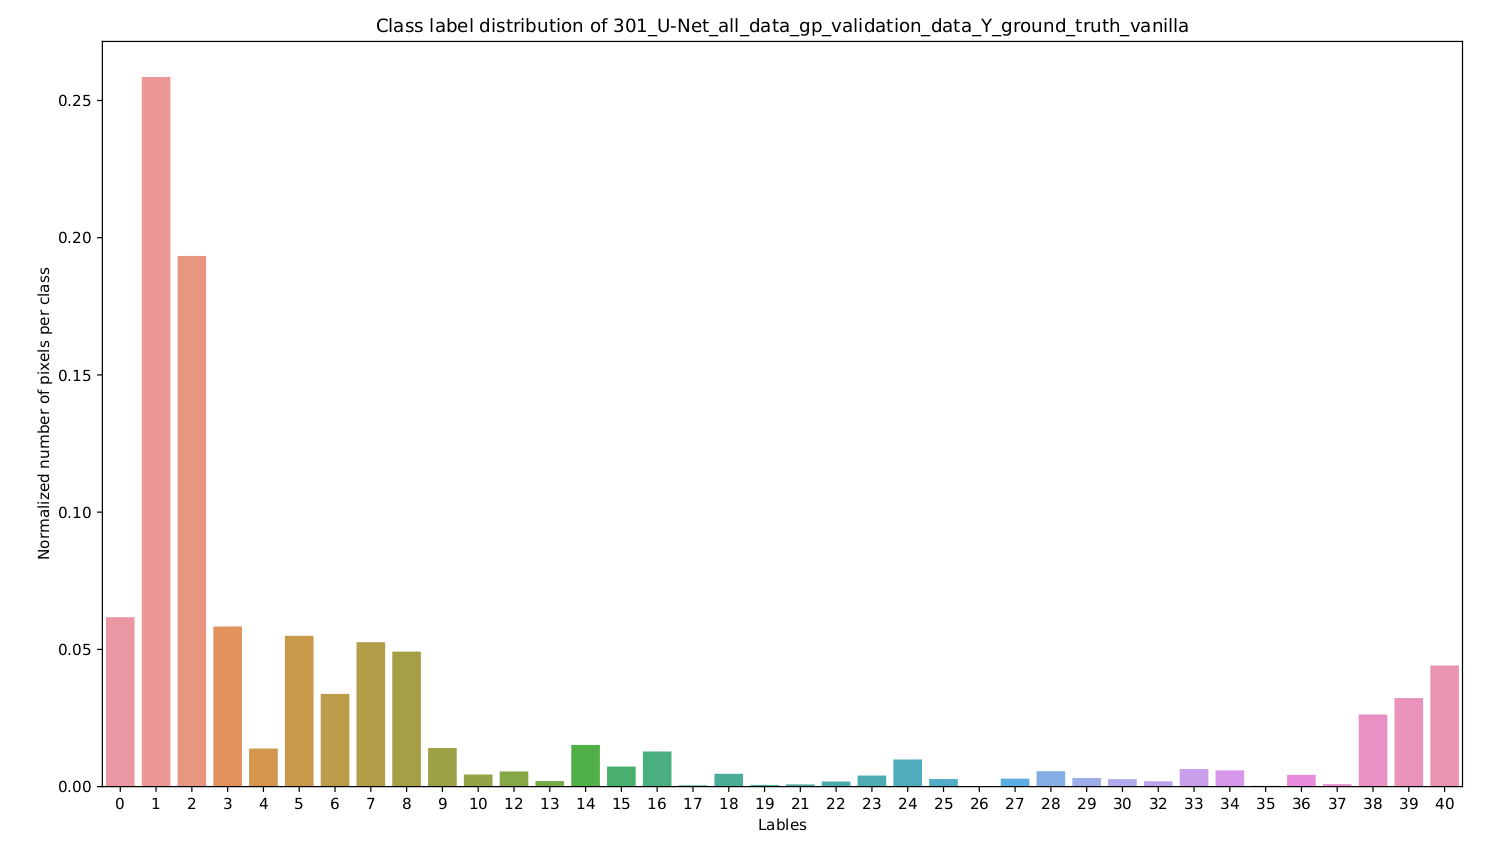
\includegraphics[width=16cm]{images/Y_ground_truth_vanilla.png}
		\caption{Per class pixel distribution of the ground truth pixel class label}
		\label{fig:y_gt_vanilla}
	\end{figure}

	\begin{figure}
		\centering
		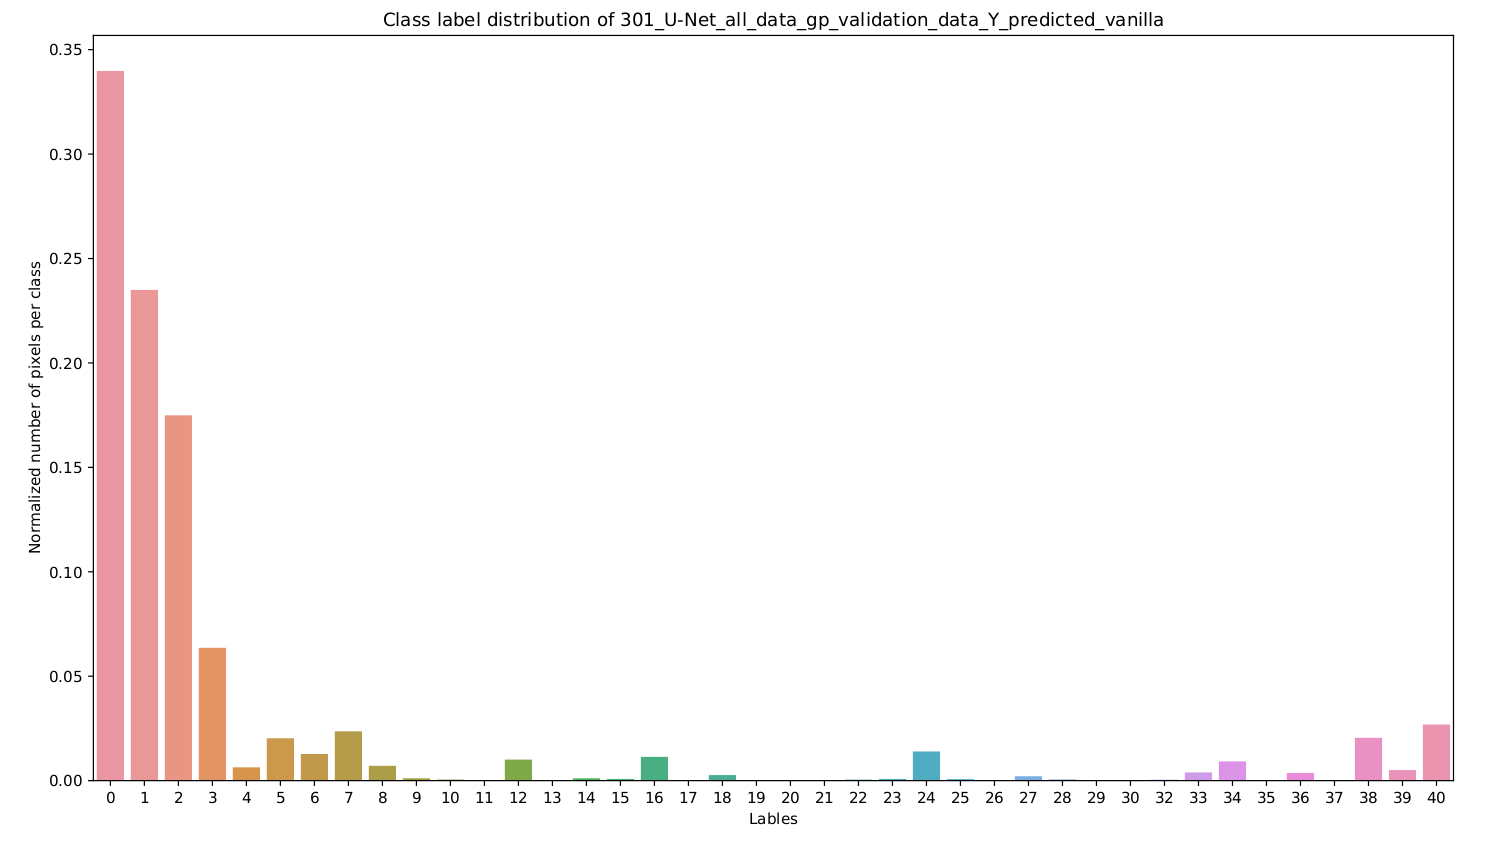
\includegraphics[width=16cm]{images/Y_predicted_vanilla.png}
		\caption{Per class pixel distribution of the predicted pixel class label}
		\label{fig:y_predi_vanilla}
	\end{figure}    

    \subsection{Experiment1.2: U-Net temporally fused gp model}
    
    { \bf Distance and covariance matrix}
    
    Ordered set of images
    
    \begin{figure}
    	\centering
    	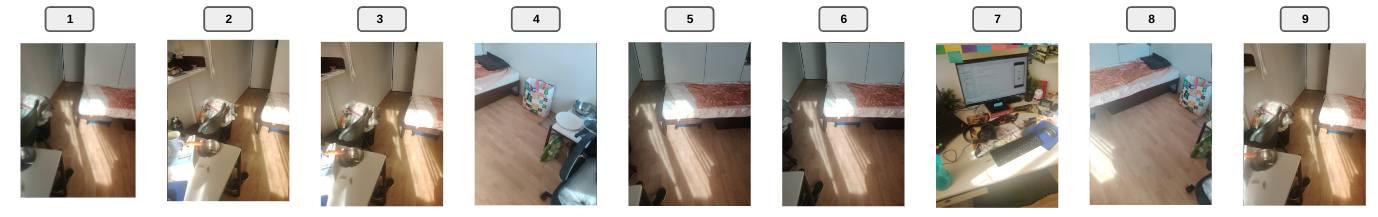
\includegraphics[width=12cm]{images/ordered_images.jpg}
    	\caption{Ordered set of images}
    	\label{fig:ordered set of images}
    \end{figure}
	
    \begin{figure}
		\centering
		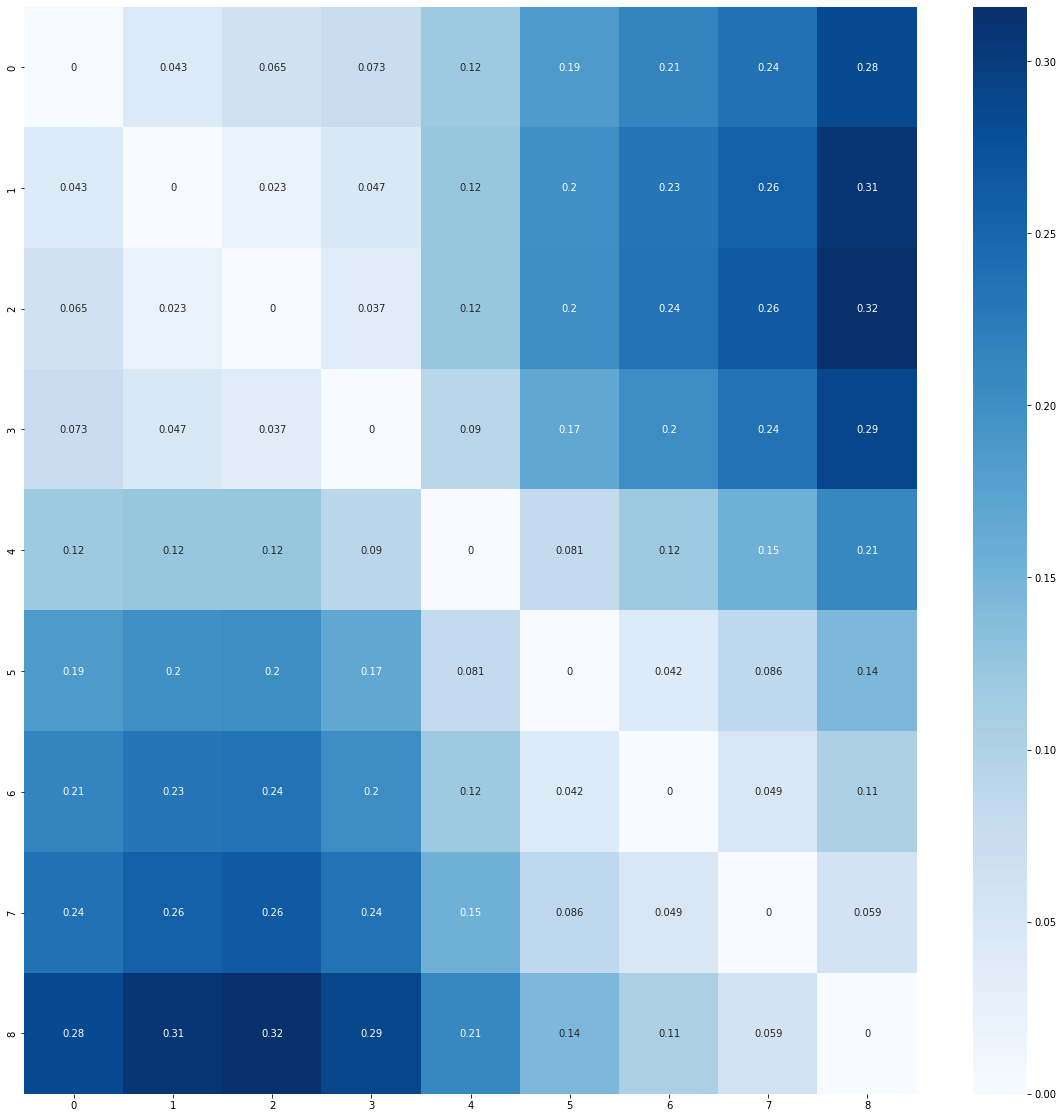
\includegraphics[width=12cm]{images/ordered_D.png}
		\caption{Distance matrix depicted as heatmap}
		\label{fig:ordered set D}
	\end{figure}  
    
    \begin{figure}
    	\centering
    	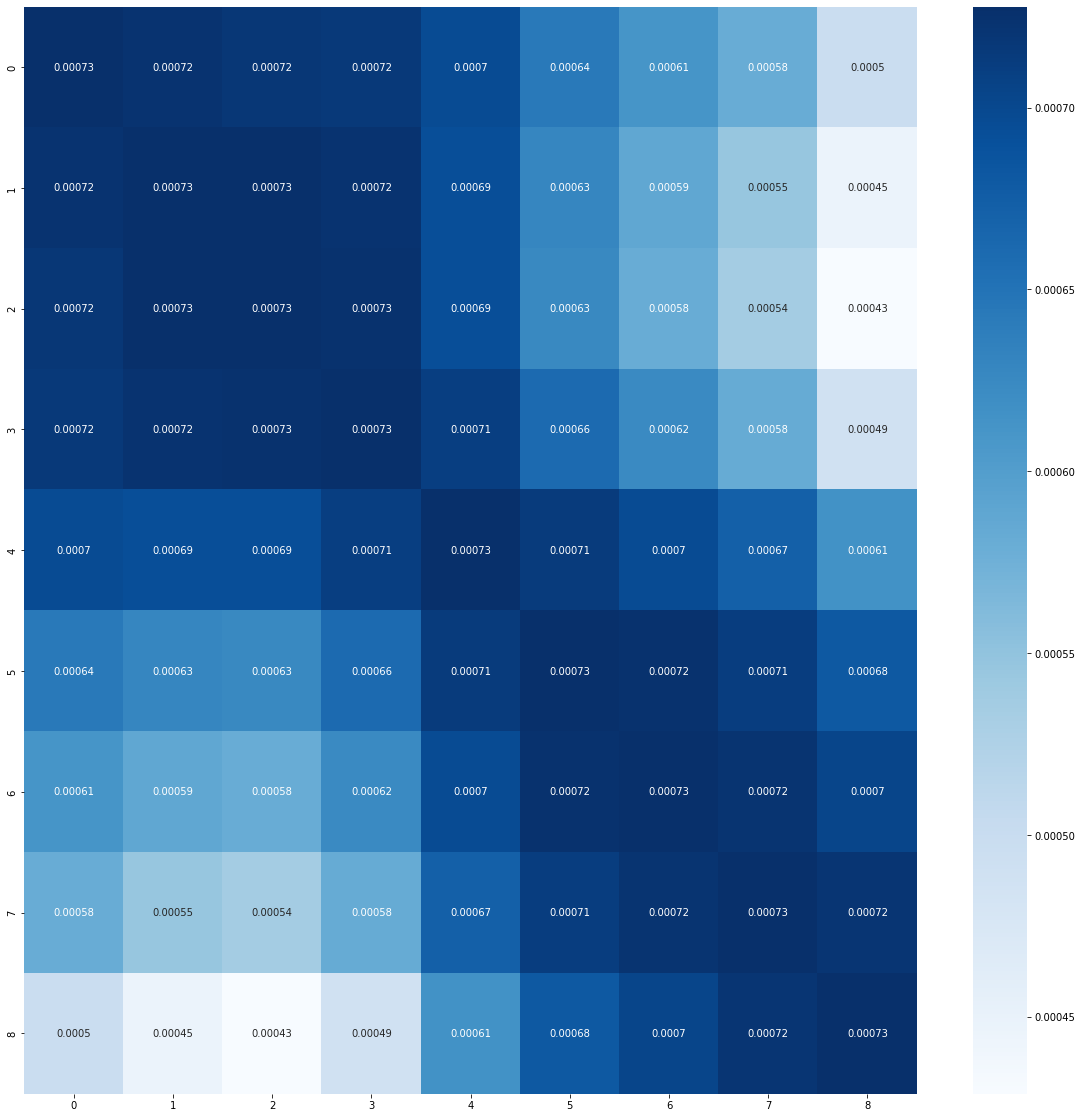
\includegraphics[width=12cm]{images/ordered_K.png}
    	\caption{Kernel matrix depicted as heatmap}
    	\label{fig:ordered set of K}
    \end{figure}
	
    \begin{figure}
		\centering
		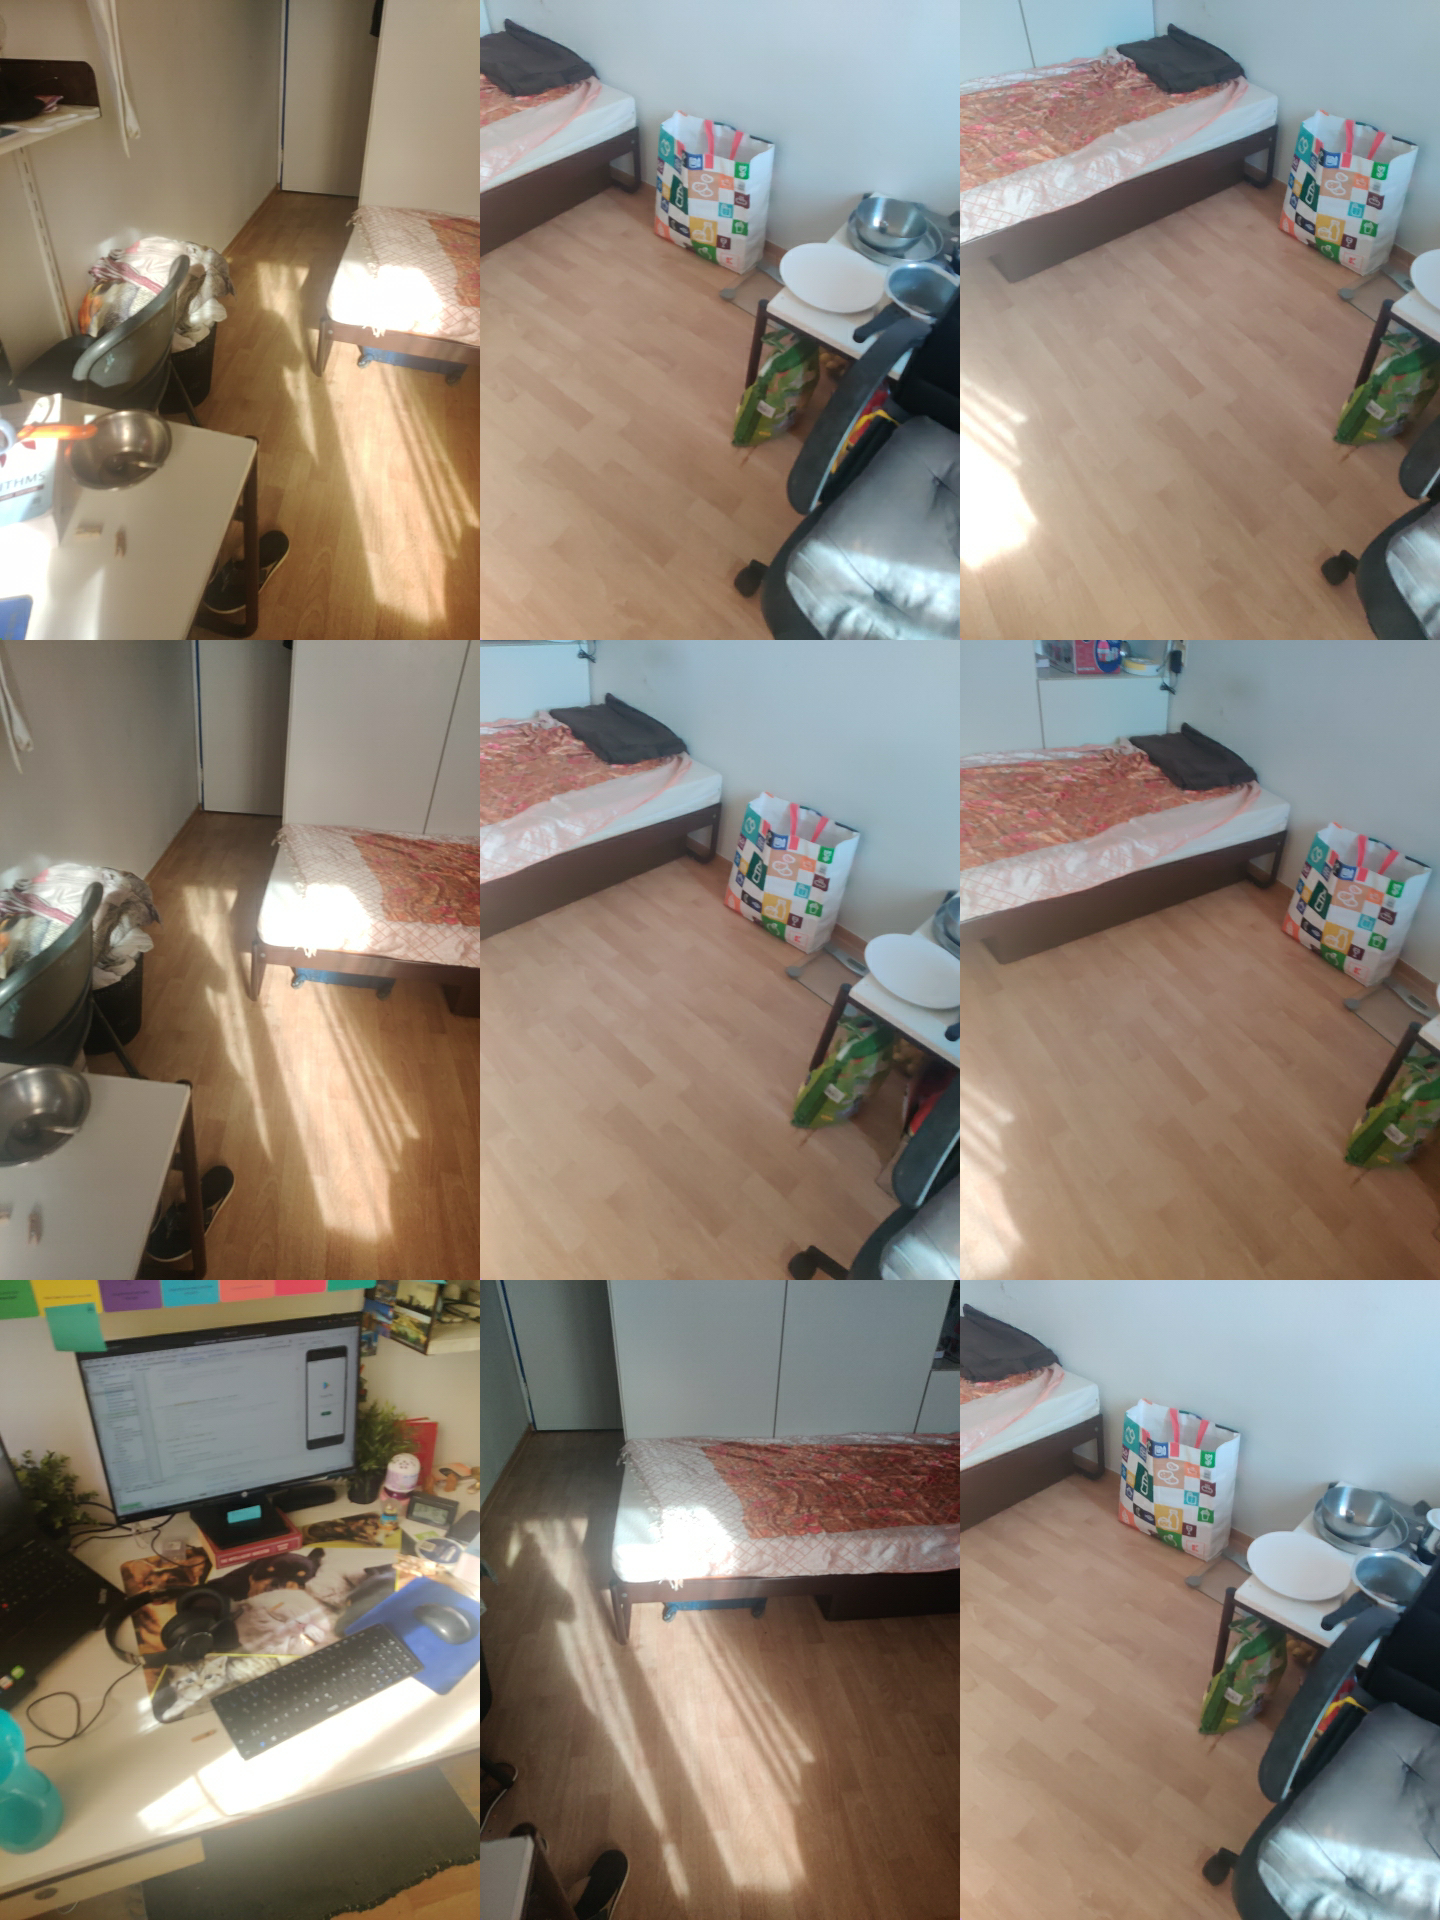
\includegraphics[width=12cm]{images/unordered_images.jpg}
		\caption{Ordered set of images}
		\label{fig:unordered set of images}
	\end{figure}
	
	\begin{figure}
		\centering
		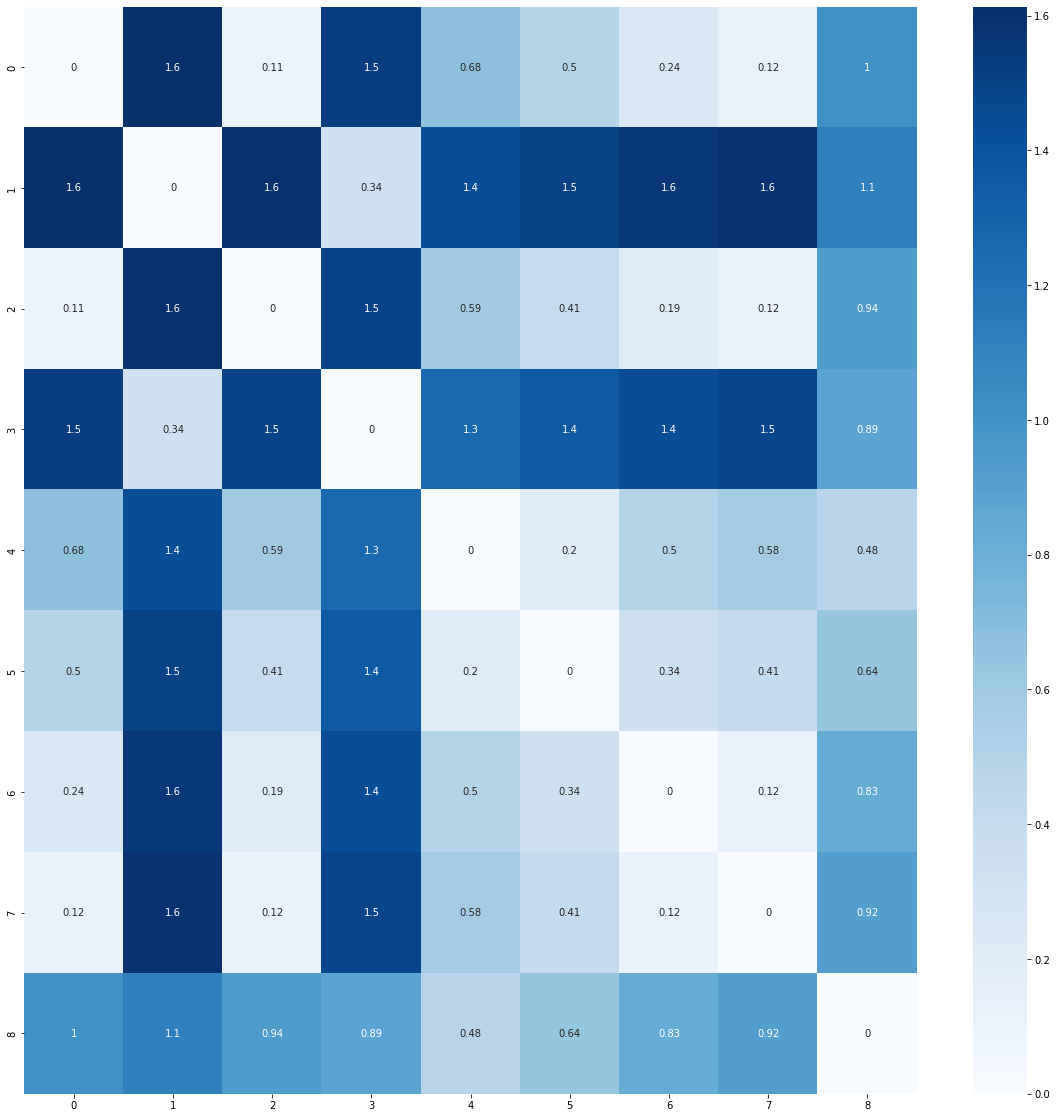
\includegraphics[width=12cm]{images/unordered_D.png}
		\caption{Distance matrix depicted as heatmap}
		\label{fig:unordered set K}
	\end{figure}  
	
	\begin{figure}
		\centering
		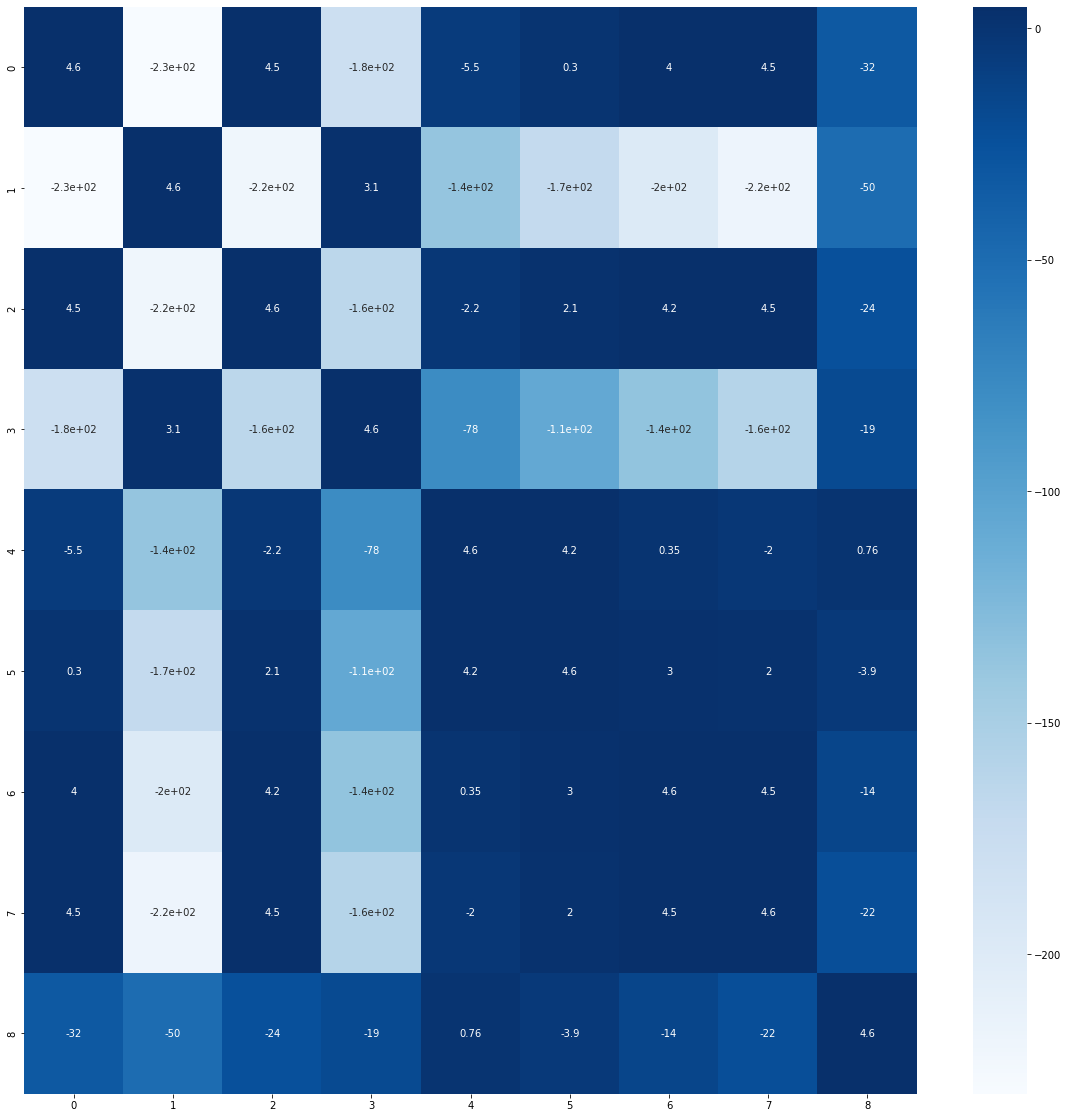
\includegraphics[width=12cm]{images/unordered_K.png}
		\caption{Kernel matrix depicted as heatmap}
		\label{fig:unordered set of K}
	\end{figure}

    { \bf Results of the experiment}
    
    \begin{center}
    	\begin{tabular}{ | l | p{12cm} |}
    		\hline
    		
    		\cellcolor{purple!30}Metric & \cellcolor{purple!30}Value \\ \hline
    		Pixel Accuracy & 0.5184 \\ \hline
    		Pixel Mean accuracy & 0.1679  \\ \hline
    		meanIOU & 0.1161 \\ \hline
    		IoU & [1.7087e-01, 5.1271e-01, 5.9998e-01, 2.1256e-01, 4.1160e-01, 1.5834e-01,
    		3.8634e-02, 2.3669e-01, 1.6056e-01, 1.1568e-01, 7.9677e-02, 1.0454e-02,
    		2.4003e-02, 0.0000e+00, 1.2199e-01, 4.3193e-02, 3.3956e-01, 6.6473e-02,
    		1.4712e-01, 2.8003e-03, 6.0475e-05, 2.6127e-01, 5.7962e-02, 0.0000e+00,
    		3.4611e-04, 1.6519e-02, 0.0000e+00, 4.3417e-04, 4.4221e-02, 6.6478e-03,
    		1.2108e-02,        nan, 5.3272e-02, 5.8480e-02, 2.2352e-01, 4.2175e-02,
    		8.4644e-02, 1.1630e-04, 4.9106e-02, 1.0338e-01, 1.7687e-01] \\ \hline
    		FwIoU & 0.3497 \\ \hline
    		\hline
    	\end{tabular}
    \end{center}
	
	\begin{figure}
		\centering
		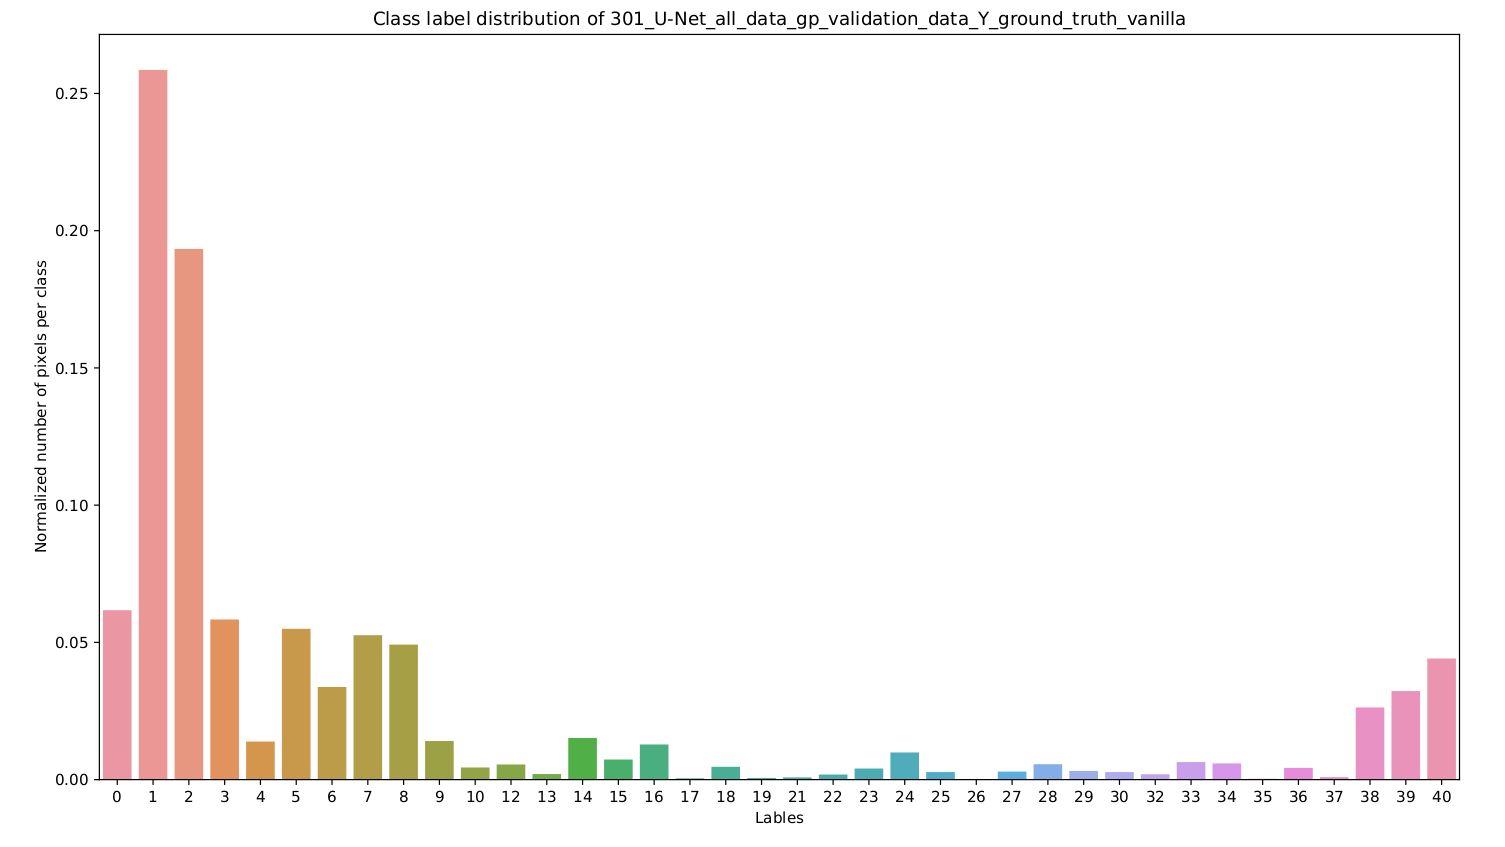
\includegraphics[width=16cm]{images/Y_ground_truth_gp.png}
		\caption{Per class pixel distribution of the ground truth pixel class label for gp model}
		\label{fig:y_gt_gp}
	\end{figure}
	
	\begin{figure}
		\centering
		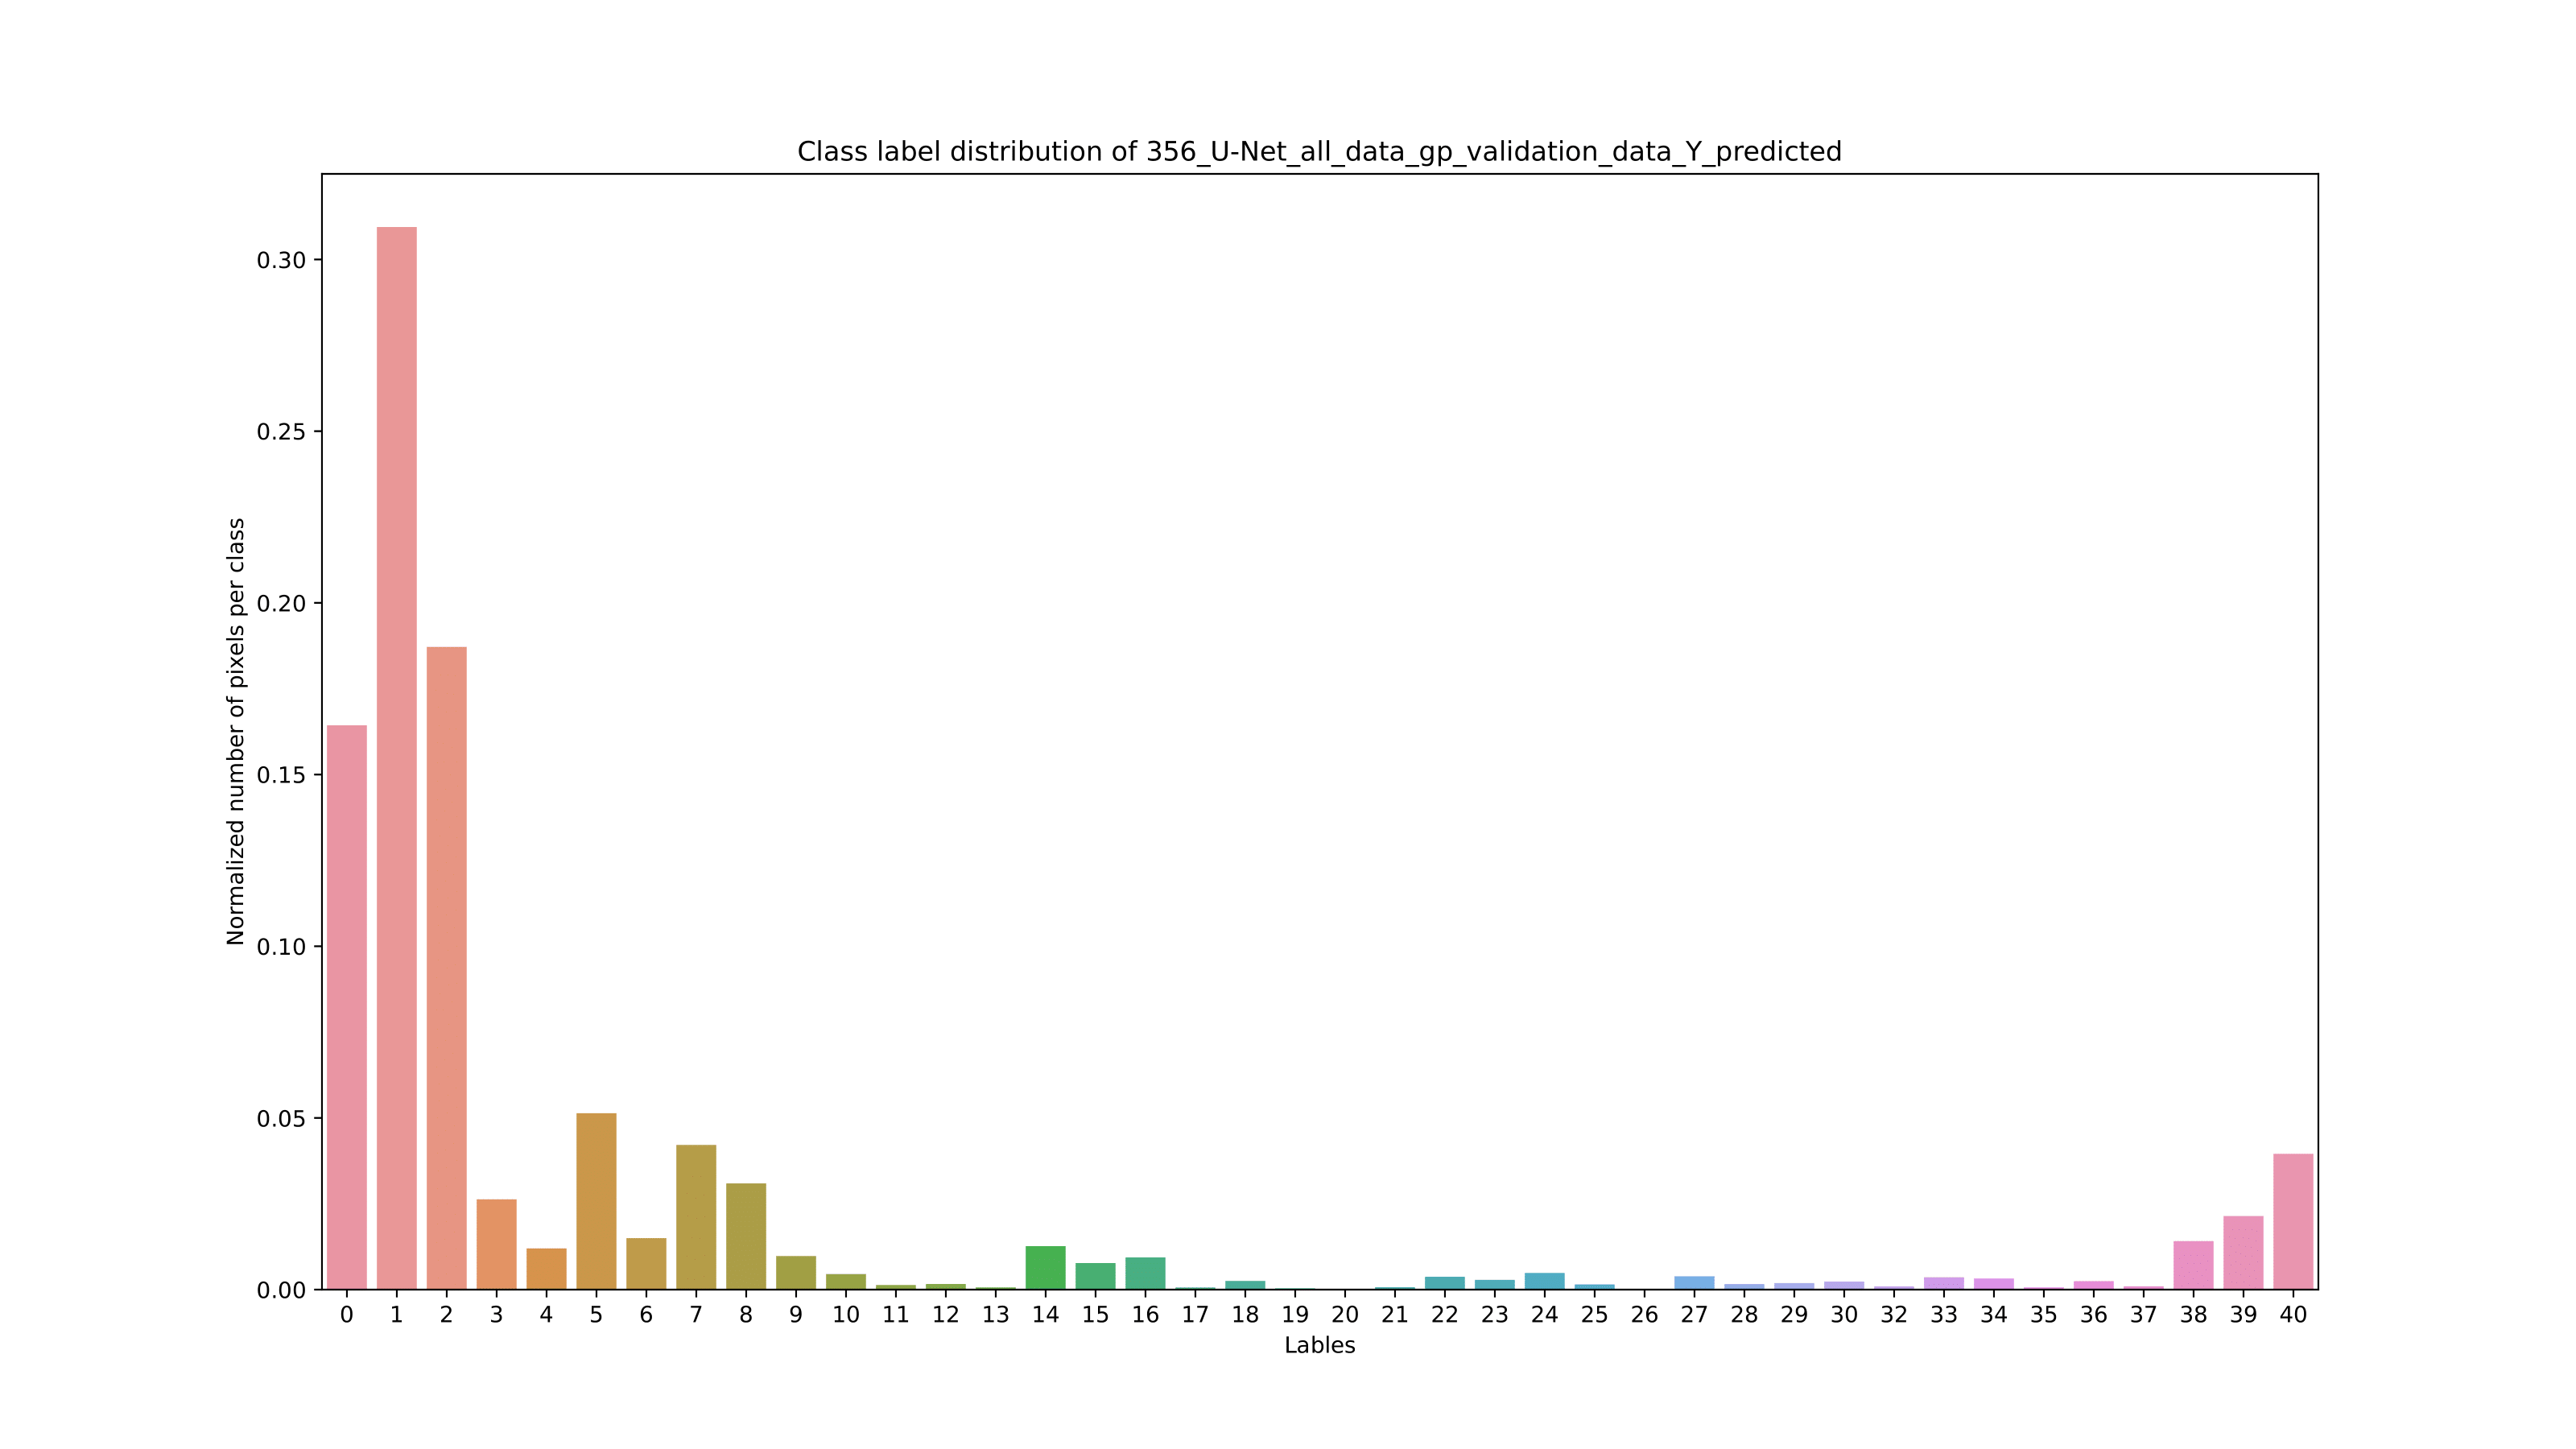
\includegraphics[width=16cm]{images/Y_predicted_gp.png}
		\caption{Per class pixel distribution of the predicted pixel class label for gp model}
		\label{fig:y_predi_gp}
	\end{figure}

    \subsection{Experiment1.3: U-Net temporally fused lstm model}
    
    \begin{center}
    	\begin{tabular}{ | l | p{12cm} |}
    		\hline
    		
    		\cellcolor{purple!30}Metric & \cellcolor{purple!30}Value \\ \hline
    		Pixel Accuracy & 0.5601 \\ \hline
    		Pixel Mean accuracy & 0.2254  \\ \hline
    		meanIOU & 0.145 \\ \hline
    		IoU & [0.2664, 0.6187, 0.6561, 0.0875, 0.4232, 0.1989, 0.0567, 0.1796, 0.2832,
    		0.1905, 0.0258, 0.2313, 0.0013, 0.0000, 0.0681, 0.1169, 0.2300, 0.0685,
    		0.1384, 0.0182, 0.0000, 0.0600, 0.1695, 0.0515, 0.0000, 0.3135, 0.0000,
    		0.0000, 0.0069, 0.0335, 0.1894,    nan, 0.0804, 0.1759, 0.1104, 0.1517,
    		0.0053, 0.0996, 0.1119, 0.1184, 0.2613] \\ \hline
    		FwIoU & 0.3996 \\ \hline
    		\hline
    	\end{tabular}
    \end{center}
	
	\begin{figure}
		\centering
		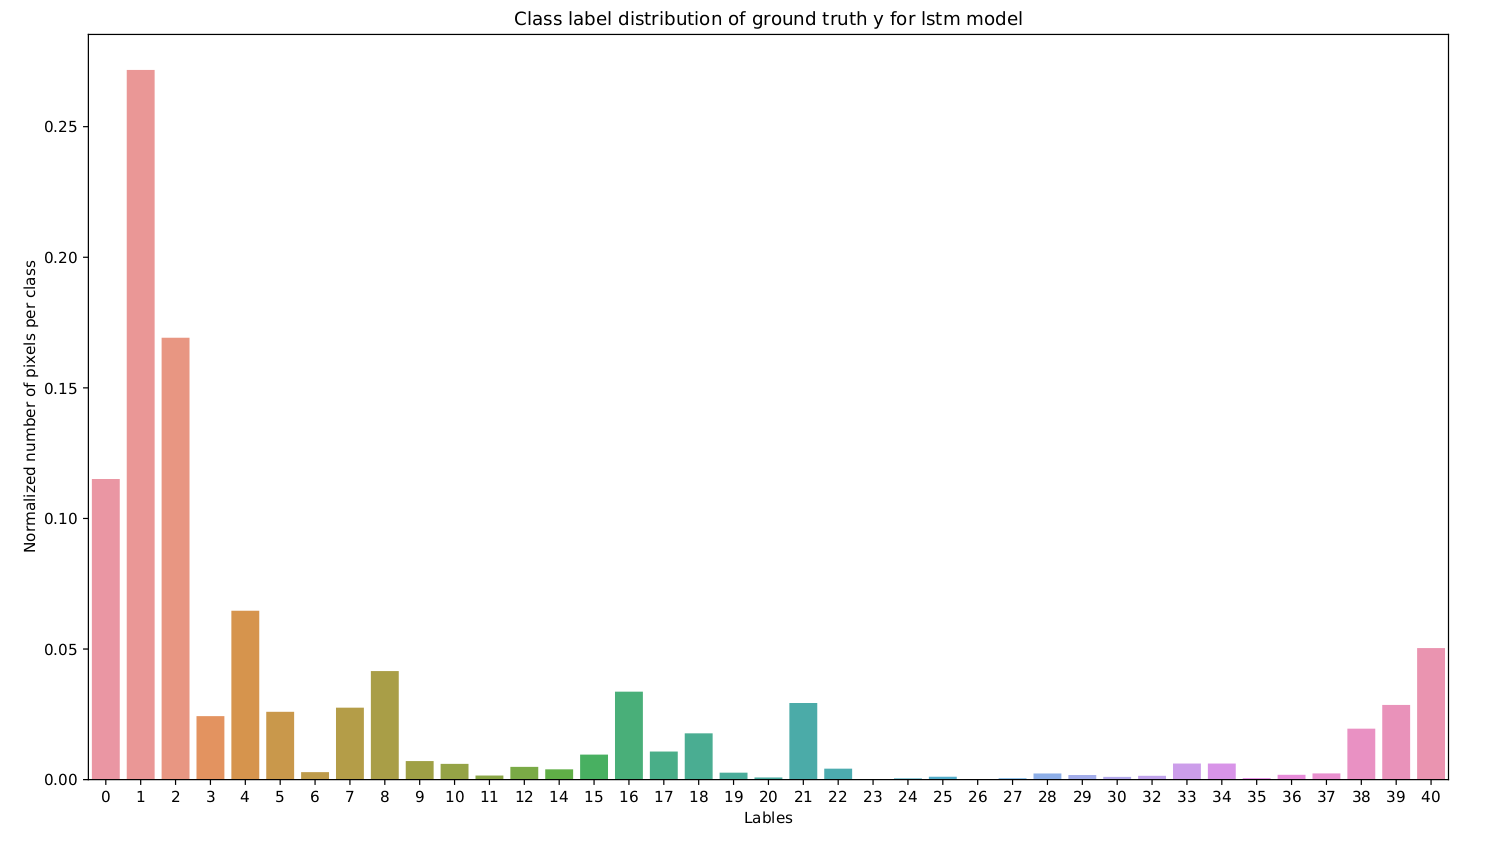
\includegraphics[width=16cm]{images/Y_ground_truth_lstm.png}
		\caption{Per class pixel distribution of the ground truth pixel class label for lstm model}
		\label{fig:y_gt_lstm}
	\end{figure}
	
	\begin{figure}
		\centering
		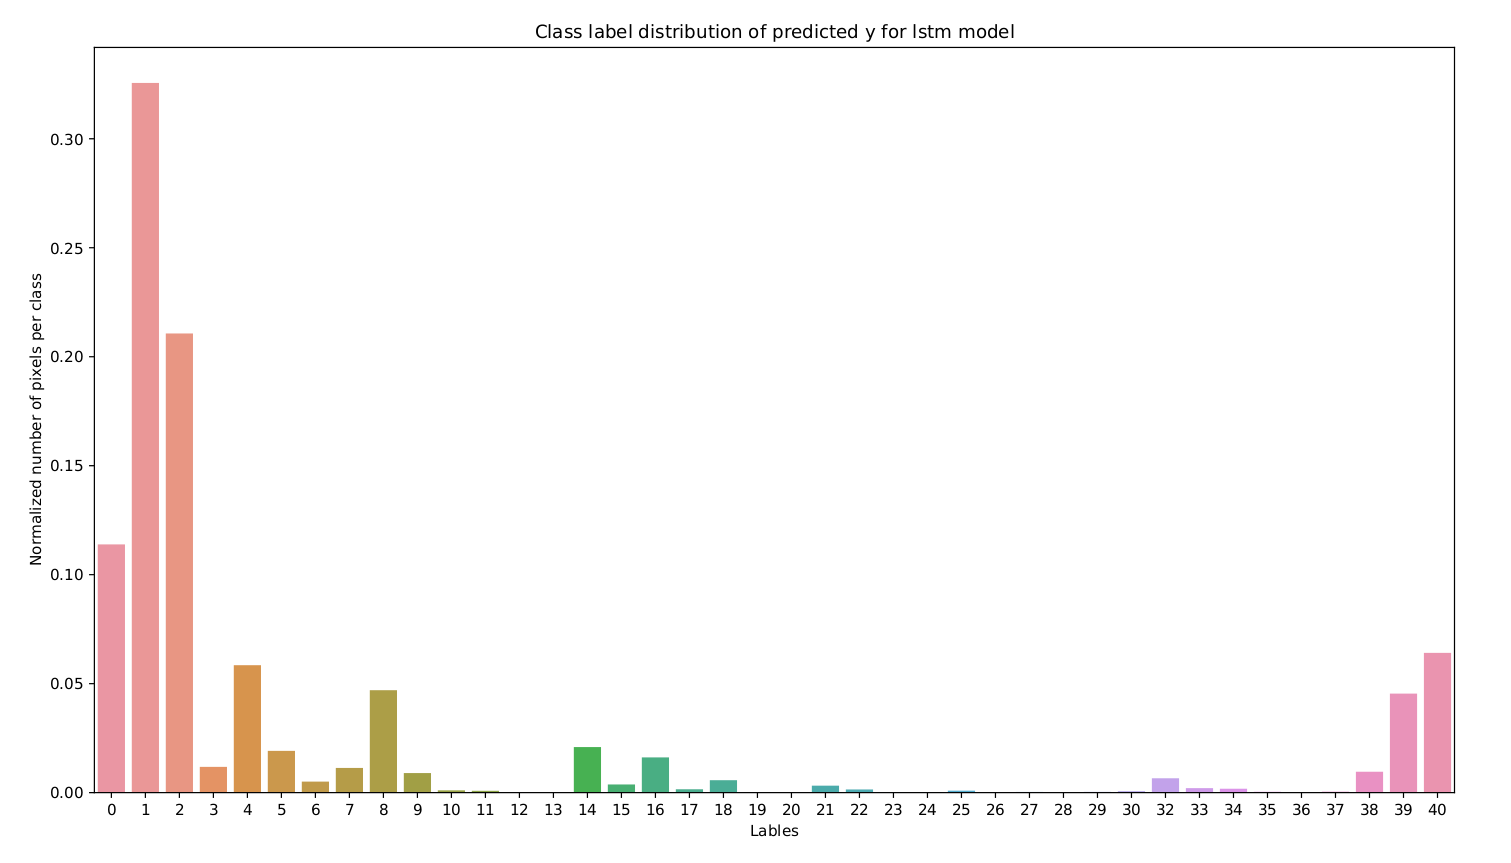
\includegraphics[width=16cm]{images/Y_predicted_lstm.png}
		\caption{Per class pixel distribution of the predicted pixel class label for lstm model}
		\label{fig:y_predi_lstm}
	\end{figure}
	
	\subsection{Temporal fusion on a continuous sequence data}
	
	\begin{figure}
		\centering
		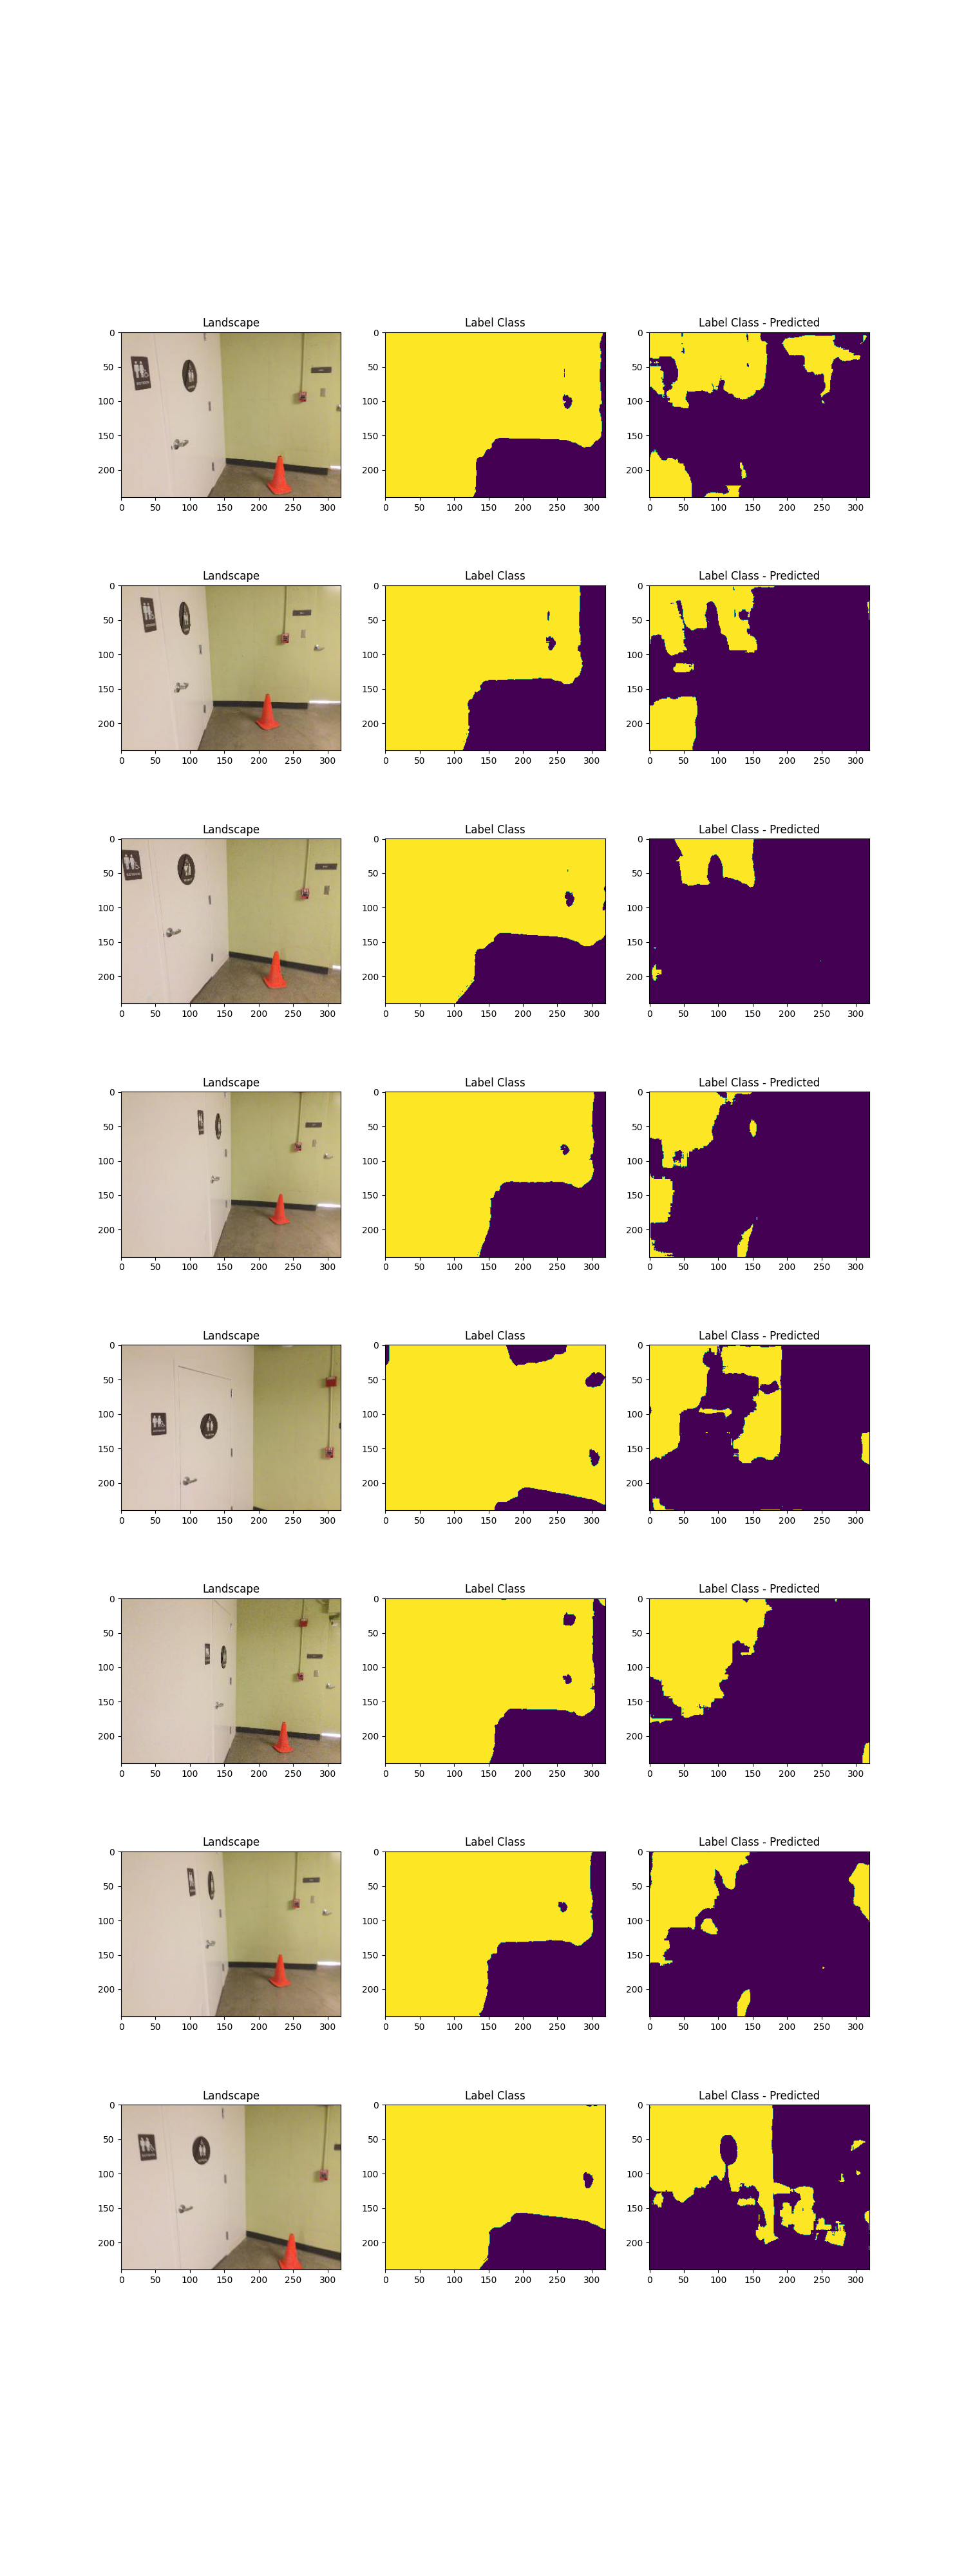
\includegraphics[width=16cm]{images/output_vanilla.png}
		\caption{Plotting of raw input image, ground truth and vanilla model predicted output on a continuous sequence data}
		\label{fig:output_vanilla}
	\end{figure}
	
	\begin{table}
	\begin{center}
		\begin{tabular}{ | l | p{12cm} |}
			\hline
			
			\cellcolor{purple!30}Metric & \cellcolor{purple!30}Value \\ \hline
			Pixel Accuracy & 0.4342 \\ \hline
			Pixel Mean accuracy & 0.6232  \\ \hline
			meanIOU & 0.145 \\ \hline
			IoU & [0.2737, 0.2809] \\ \hline
			FwIoU & 0.2793 \\ \hline
			\hline
		\end{tabular}
		\caption{Performance of Vanilla model with respect to different metric and two classes}
		\label{table:Vanilla_conti_seq}
	\end{center}
	\end{table}
	
	\begin{figure}
		\centering
		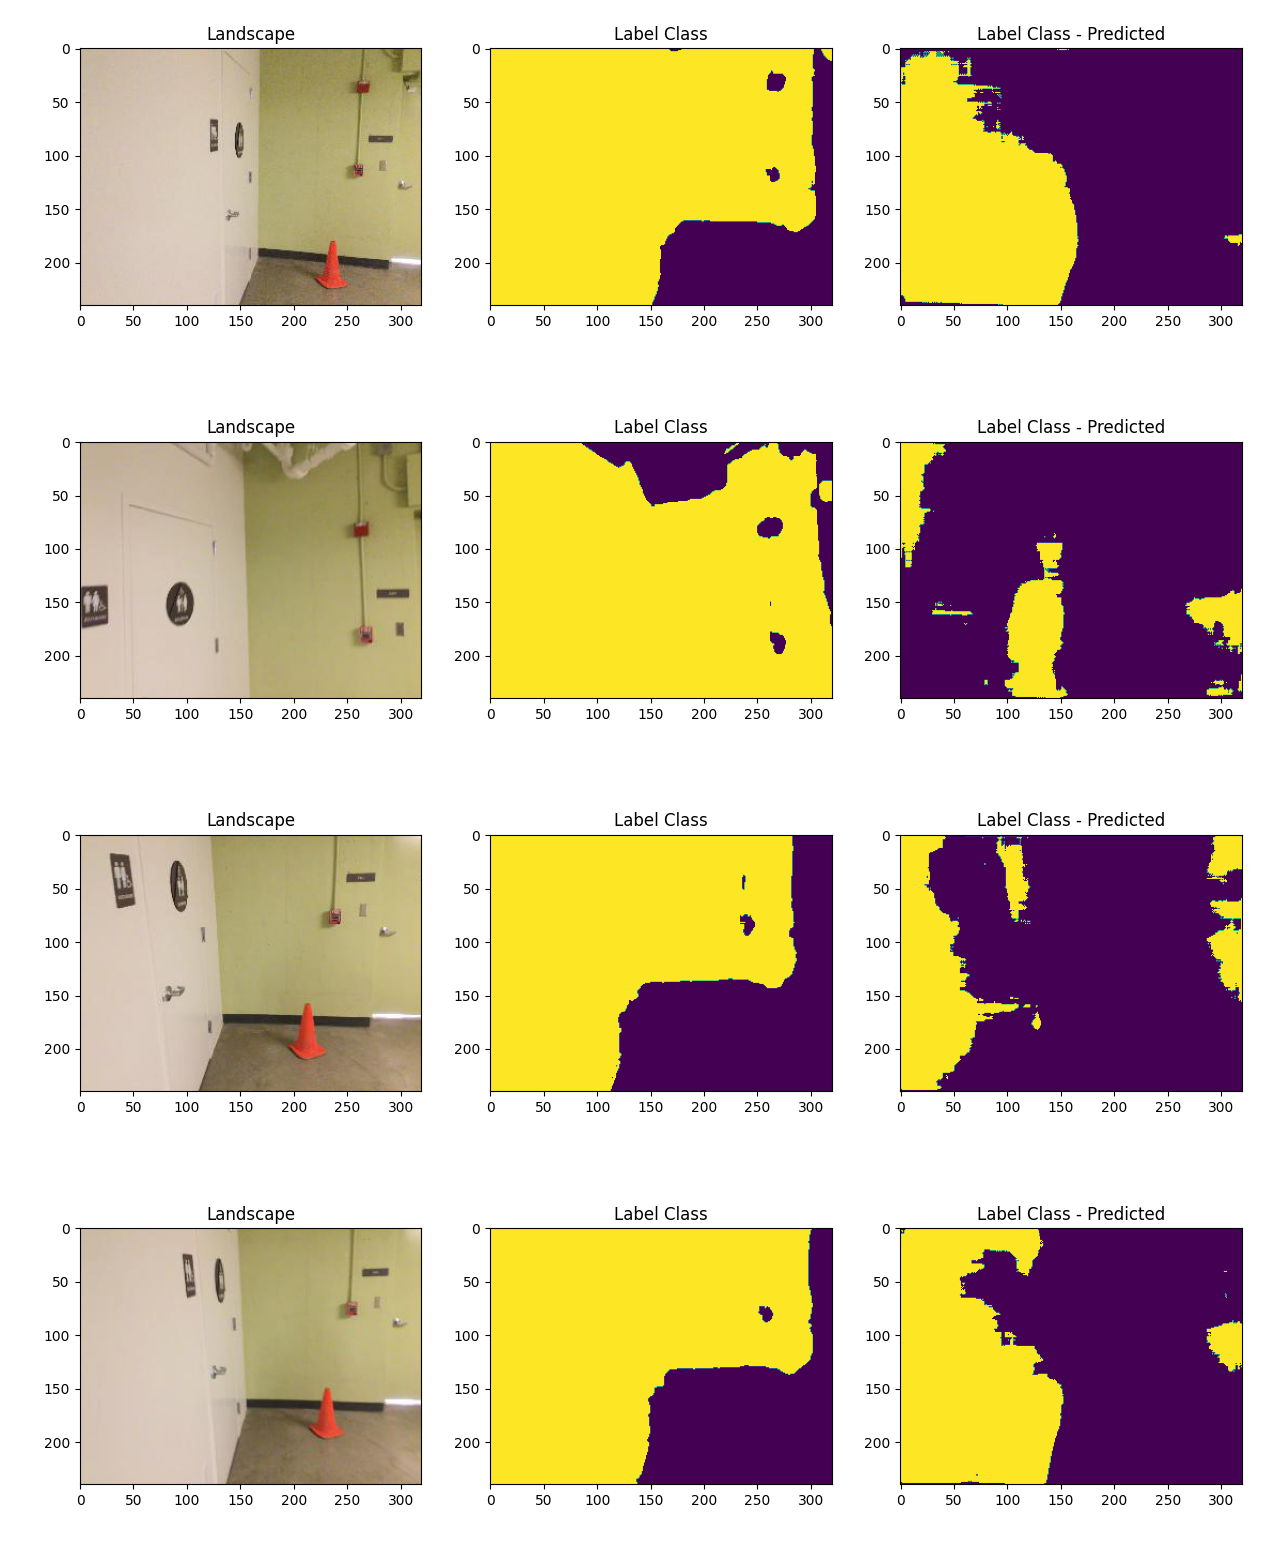
\includegraphics[width=16cm]{images/output_gp.png}
		\caption{Plotting of raw input image, ground truth and GP model predicted output on a continuous sequence two class data }
		\label{fig:output_gp}
	\end{figure}
	
	\begin{table}
	\begin{center}
		\begin{tabular}{ | l | p{12cm} |}
			\hline
			
			\cellcolor{purple!30}Metric & \cellcolor{purple!30}Value \\ \hline
			Pixel Accuracy & 0.3764 \\ \hline
			Pixel Mean accuracy & 0.5625  \\ \hline
			meanIOU & 0.2318 \\ \hline
			IoU & [0.2377, 0.2259] \\ \hline
			FwIoU & 0.2284 \\ \hline
			\hline
		\end{tabular}
		\caption{Performance of GP model with respect to different metric and two classes}
		\label{table:GP_conti_seq}
	\end{center}
	\end{table}
	

	\begin{figure}
		\centering
		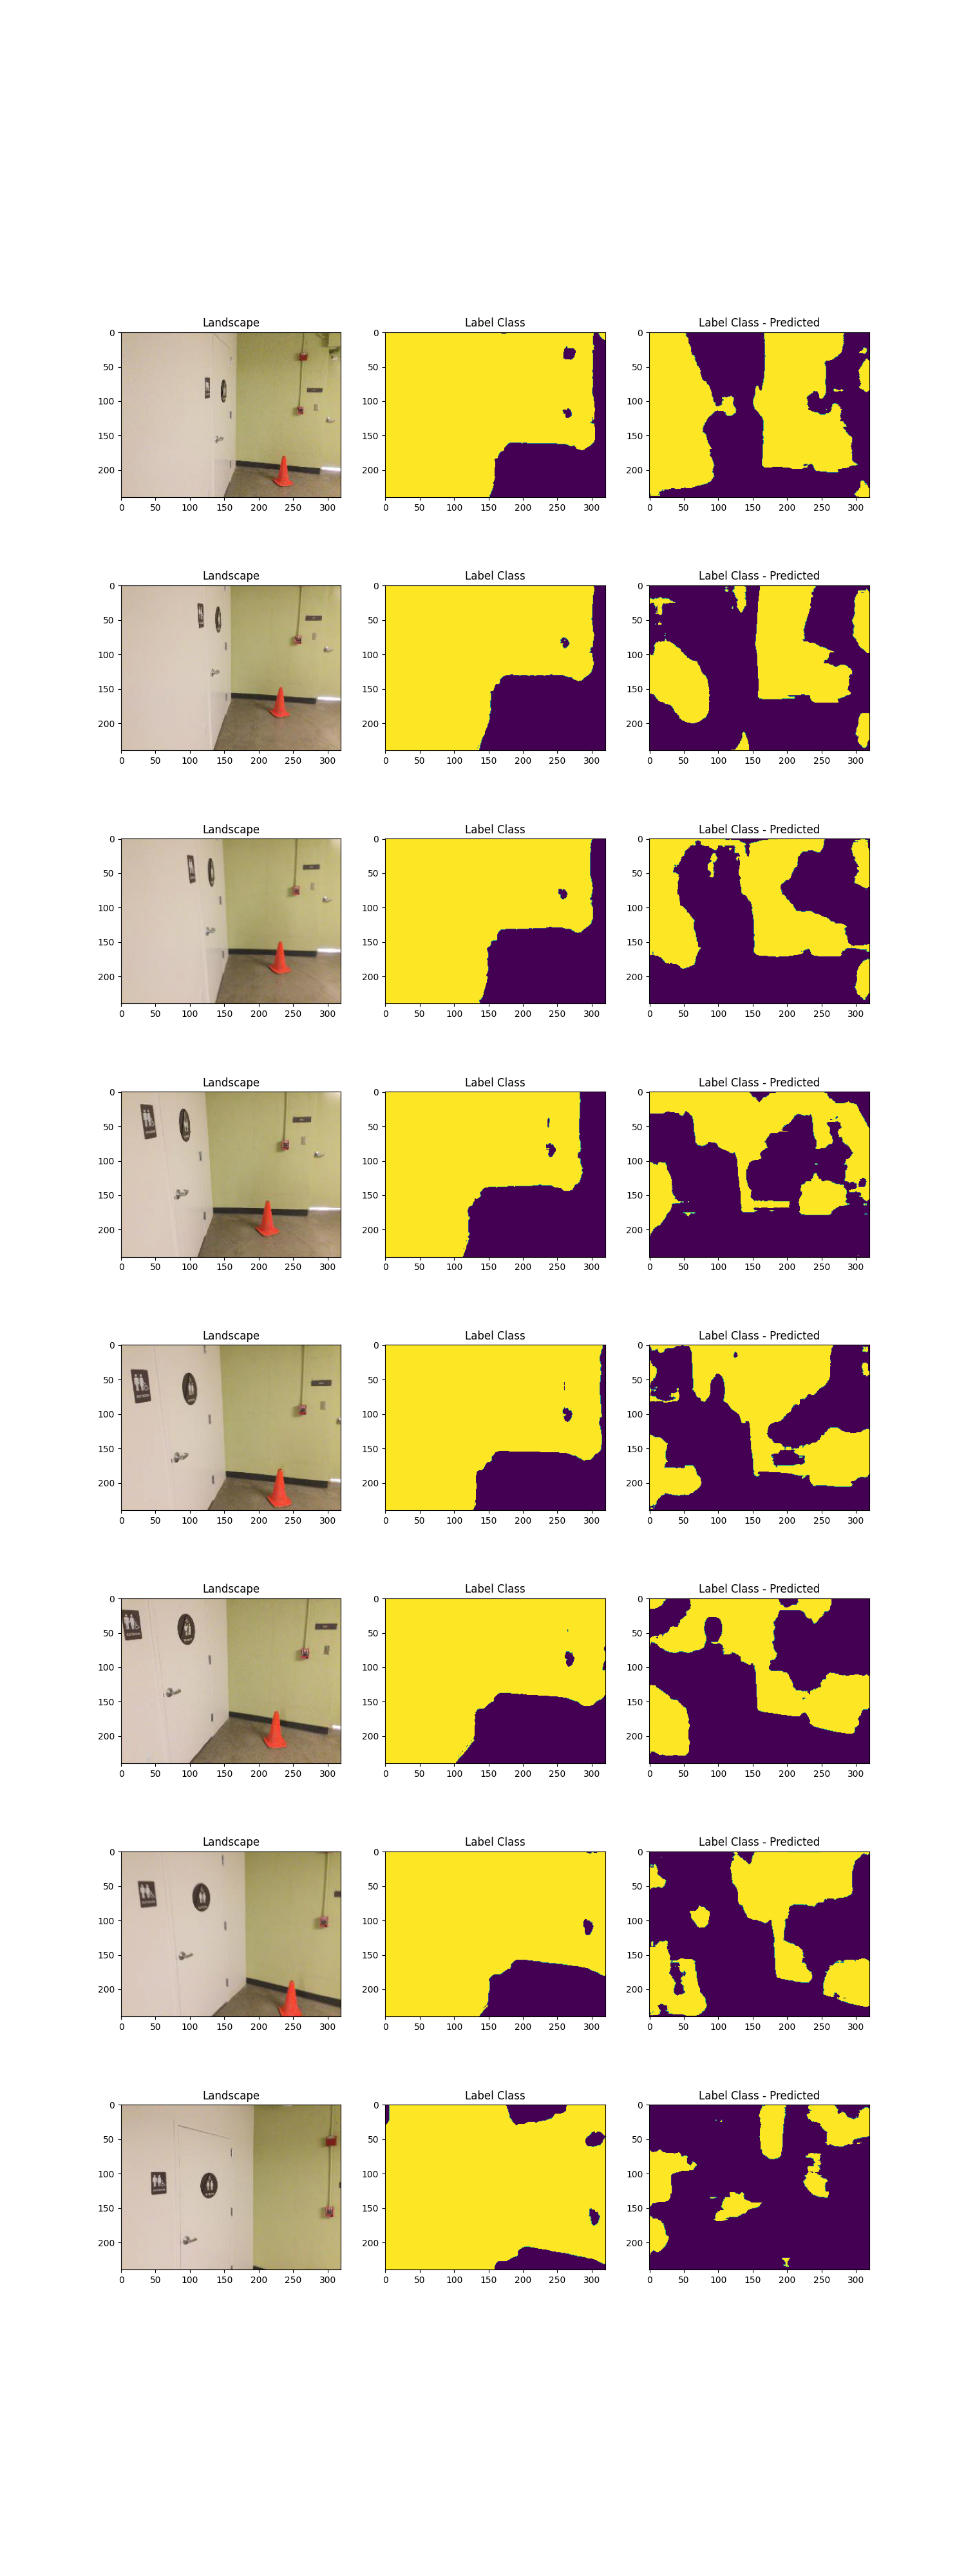
\includegraphics[width=16cm]{images/output_lstm.png}
		\caption{Plotting of raw input image, ground truth and lstm model predicted output on a continuous sequence two class data}
		\label{fig:output_lstm}
	\end{figure}
	
	\begin{table}
	\begin{center}
		\begin{tabular}{ | l | p{12cm} |}
			\hline
			
			\cellcolor{purple!30}Metric & \cellcolor{purple!30}Value \\ \hline
			Pixel Accuracy & 0.4496 \\ \hline
			Pixel Mean accuracy & 0.5301  \\ \hline
			meanIOU & 0.2832 \\ \hline
			IoU & [0.2135, 0.3530] \\ \hline
			FwIoU & 0.3221 \\ \hline
			\hline
		\end{tabular}
		\caption{Performance of LSTM model with respect to different metric and two classes}
		\label{table:LSTM_conti_seq}
	\end{center}
	\end{table}
	
    \subsection{RQ3.1: Which fusion method is good for the scannet data?}
    \subsection{RQ3.2: Which fusion method is good for the virtual kitti data?}
    \subsection{RQ3.3: Which fusion method is good for the VIODE data?}
    
\end{document}
